% !Mode:: "TeX:UTF-8"

\titlepage

% \begin{frame}{说在前面}
% 	\linespread{1.5}
% 	  \begin{itemize}[<+-|alert@+>]
% 	    \item \ba{箭头!箭头!箭头!}
% 	    \item \ba{画图!画图!画图!}
% 	    \item 不记得自己哪周交作业
% 	  \end{itemize}
% \end{frame}

% \begin{frame}{需要注意的问题}
% 	\linespread{1.5}
% 	  \begin{itemize}%[<+-|alert@+>]
% 	    \item L'Hospital法则
% 	    \begin{itemize}
% 	      \item \it 只能应用于“$\df{\bm{0}}{\bm{0}}$”
% 	      和“$\df{\bm{\infty}}{\bm{\infty}}$”型
% 	      \item \it 及时使用无穷小代换进行简化
% 	      \item \it 不正规的符号:\b 
% 	      $\xlongequal{\footnotesize\mbox{“L”}}$、
% 	      $\xlongrightarrow{\footnotesize\mbox{“L'Hospital法则”}}$、
% 	      $\df{\bm{0}}{\bm{0}}$、$\df{\bm{\infty}}{\bm{\infty}}$
% 	    \end{itemize}
% 	    \item Taylor公式
% 	    \begin{itemize}
% 	      \item \it Taylor多项式不包含余项
% 	      \item \it 合并同次幂的系数
% 	      \item \it 尽量按照幂次由低到高排列,最后写余项
% 	    \end{itemize}
% 	  \end{itemize}
% \end{frame}

\begin{frame}
	\linespread{1.5}
	\ba{1.求过直线$x=y=z$,且垂直于$xOy$坐标面的平面的一般式方程。}
	
	\bigskip
	
	\small 解:\it
	所求平面的法向量
	$$\bm{n}=\left|\begin{array}{ccc}
		\bm{i} & \bm{j} & \bm{k}\\
		1 & 1 & 1 \\
		0 & 0 & 1
	\end{array}\right|=(1,-1,0).$$
	直线$x=y=z$过原点,故原点位于所求平面上,从而可得其方程为
	$$x-y=0.$$
	\fin
\end{frame}

\begin{frame}
	\linespread{1.5}
	\ba{2.求点$(1,3,1)$关于平面$x+y=0$的对称点。}
	
% 	\bigskip
	
	\small 解:\it
	过点$(1,3,1)$垂直于平面$x+y=0$的直线方向为
	$$\df{x-1}1=\df{y-3}1=\df{z-1}0.$$
	其于平面的交点为$(-1,1,1)$,从而所求对称点为
	$(-3,-1,1)$。\fin
\end{frame}

\begin{frame}
	\linespread{1.5}
	\ba{3.求过点$(3,1,-2)$且过直线$\df{x-4}5=\df{y+3}2=z$的平面
	的一般式方程。}
	
	\bigskip
	
	\small 解:\it
	所求平面的法向量为
	$$\bm{n}=\left|\begin{array}{ccc}
		\bm{i} & \bm{j} & \bm{k}\\
		1 & -4 & 2 \\
		5 & 2 & 1
	\end{array}\right|=(-8,9,22).$$
	从而该平面的方程为
	$$-8x+9y+22z+59=0.$$
	\fin
\end{frame}

\begin{frame}
	\linespread{1.5}
	\ba{4.求直线$\left\{\begin{array}{l}
	  	2x-y=0, \\ 3x-y-z-9=0
	  \end{array}\right.$
	  在平面$2x-y+z=1$上的投影直线的对称式方程。}
	
	\bigskip
	
	\small 解:\it
	已知直线的方向向量为
	$$\bm{s_1}=(2,-1,0)\times(3,-1,-1)=(1,2,1).$$
	过该直线且与已知平面垂直的平面的法向量为
	$$\bm{n}_1=(1,2,1)\times(2,-1,1)=(3,1,-5).$$
	于是所求直线的方向向量为
	$$\bm{s}=(3,1,-4)\times(2,-1,1)=(-4,-13,-5).$$
\end{frame}


\begin{frame}
	\linespread{1.5}
	\ba{4.求直线$\left\{\begin{array}{l}
	  	2x-y=0, \\ 3x-y-z-9=0
	  \end{array}\right.$
	  在平面$2x-y+z=1$上的投影直线的对称式方程。}
	
	\bigskip
	
	\small 解续:\it
	
	又联立已知直线与已知平面的方程可解得$(x,y,z)=(10,20,1)$,于是可知所求直线的
	对称式方程为
	$$\df{x-10}{4}=\df{y-20}{13}=\df{z-1}{5}.$$
	\fin
\end{frame}


\begin{frame}
	\linespread{1.5}
	\ba{5.求过直线
	$\left\{\begin{array}{l}
		x+y=0\\
		x+z+1=0
	\end{array}\right.$
	且与平面$\pi:x-4y-8z+12=0$的夹角为$\pi/4$的平面方程。}\pause
	
	\bigskip
	
	\small 解续:\it 由已知,可设过已知直线的平面束方程为
	$$\lambda(x+y)+\mu(x+z+1)=0,$$
	即$(\lambda+\mu)x+\lambda y+\mu z+\mu=0.$
	由已知
	$$\cos\df{\pi}4=\df{(\lambda+\mu,\lambda,\mu)\cdot
	(1,-4,-8)}{|(\lambda+\mu,\lambda,\mu)||(1,-4,-8)|},$$
	化简可得
	$$72\lambda^2+39\lambda\mu+32\mu^2=0,$$
	该方程无解,从而可知所求平面不存在。
	\fin
\end{frame}

\begin{frame}
	\linespread{1.5}
	\ba{6.画出下列各平面所围立体的图形:
	
	(1)$x=0,y=0,z=0,x=2,y=2,3x+4y+6z=12$}
	
	\bigskip
	
	\begin{center}
		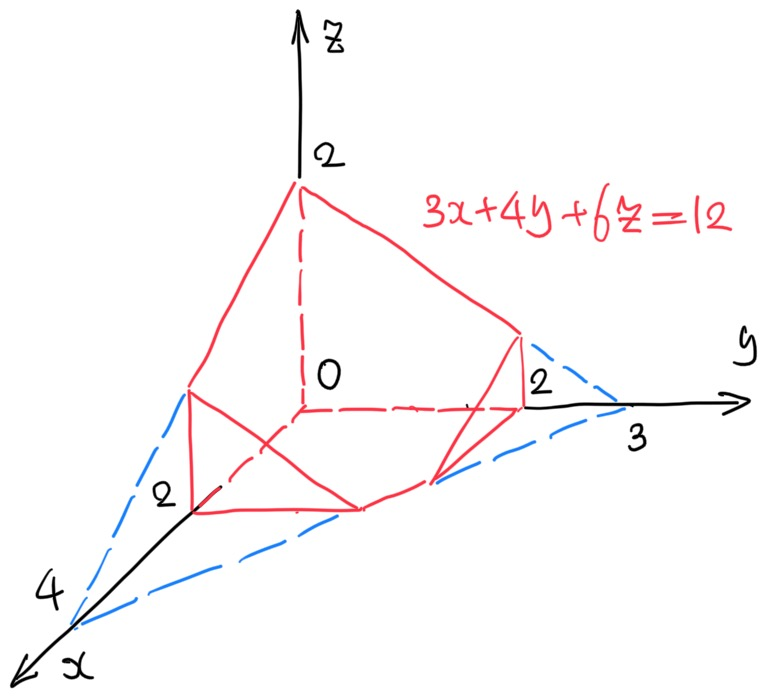
\includegraphics[width=0.6\textwidth]{./images/ch8/xyz12.jpg}
	\end{center}
\end{frame}

\begin{frame}
	\linespread{1.5}
	\ba{(2)$x+y=1,x+y+z=2,z=0,x=0,y=0$}
	
	\bigskip
	
	\begin{center}
		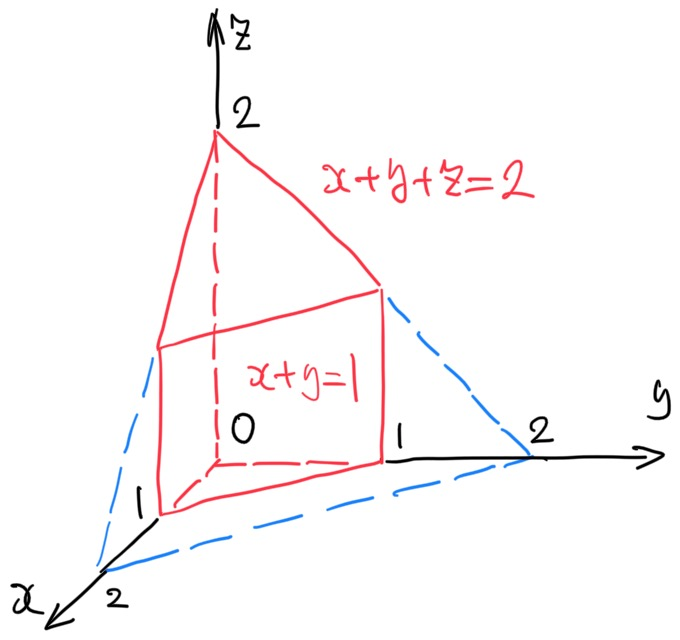
\includegraphics[width=0.6\textwidth]{./images/ch8/xyz2.jpg}
	\end{center}
\end{frame}

% \begin{frame}{出现的问题}
% 	\linespread{1.5}
% 	  \begin{itemize}%[<+-|alert@+>]
% 	    \item 作业进度慢!
% 	    \item 概念问题
% 	    \begin{itemize}
% 	      \item \b\it 幂级数展开不熟练
% 	      \item \b\it Maclaurin级数和关于$(x-x_0)$的幂级数分不清
% 	    \end{itemize}
% 	    \item 过程不规范或不完整
% 	    \begin{itemize}
% 	      \item \b\it 求收敛域要单独讨论端点的敛散性
% 	      \item \b\it 相同幂次的项要合并,并按幂次从小到大排列
% 	      \item \b\it 书写潦草随意\pause
% 	    \end{itemize}
% 	    \item \ba{雷同!!!}
% 	  \end{itemize}
% \end{frame}

% \begin{frame}
% 	\linespread{1.5}
% 	\ba{3.设$D$是由曲线$y=\sin x+1$与三条直线$x=0,x=\pi,y=0$
% 	所围成的曲边梯形,求$D$绕$x$轴旋转一周所围成的旋转体的体积。
% 	}
% 	\pause
% 	
% % 	\bigskip
% 	
% 	\begin{columns}
% 		\begin{column}{.5\textwidth}
% 			\begin{center}
% 				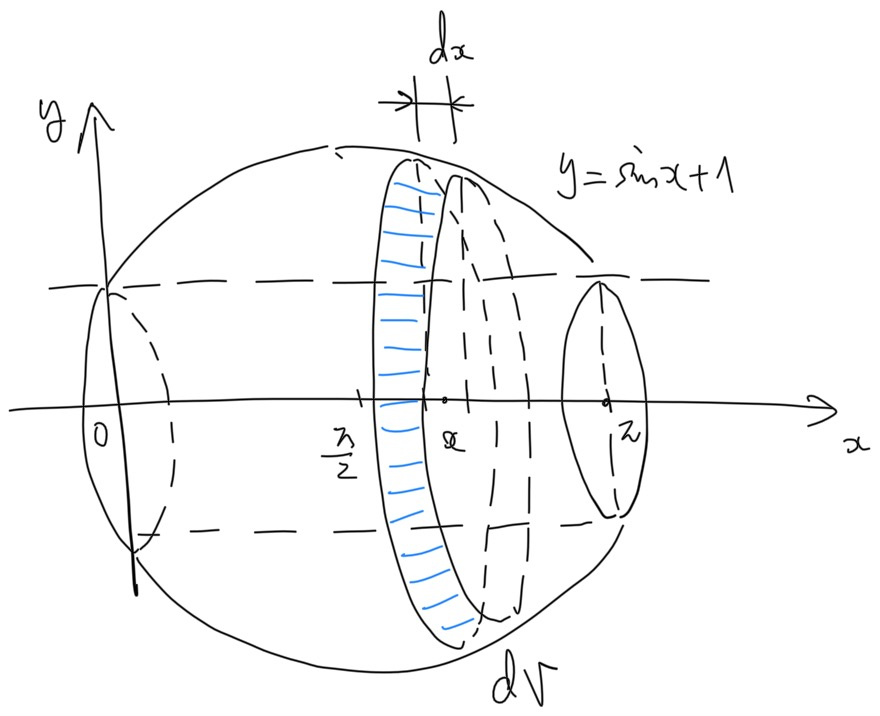
\includegraphics[width=.9\textwidth]{./images/ch6/sinx1cs.jpg}
% 		% 		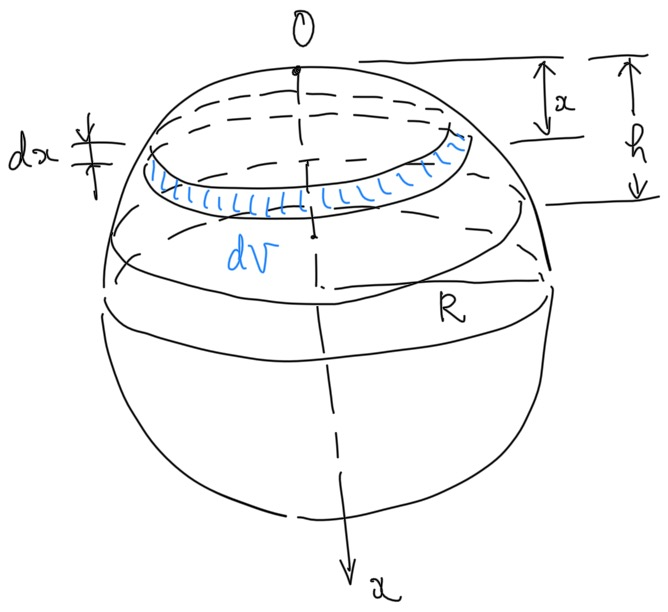
\includegraphics[width=6cm]{./images/ch6/topSp.jpg}
% 			\end{center}		
% 		\end{column}
% 		\begin{column}{.5\textwidth}
% 			\small 解:\it
% 			如图,体积微元$\d V=\pi y^2\d x$,	故所求体积
% 			$$
% 				V=\dint_0^{\pi}\pi(\sin x+1)^2\d x=\df32\pi^2.
% 			$$
% 		\end{column}
% 	\end{columns}
% \end{frame}